\documentclass{article}
\usepackage{amsmath}
\usepackage{graphicx}
\usepackage{float}
\graphicspath{ {.} }

\title{Kinetic And Potential Energy}
\author{Alex Katsenelenbogen}

\setlength{\voffset}{-0.75in}

\begin{document}
\begin{center}
      \Large\textbf{Kinetic and Potential Energy}\\
      \large\textit{Prepared by Alex Katsenelenbogen}
 \end{center}
 
 
\textbf{Problem 1:}
In the below roller coaster, the cart of mass 10kg will leave from A with a starting speed of 0 m/s. In the following problems you will consider potential and kinetic energy at different points.
To help with this exercise, you should first consider that the total amount of energy remains constant. So, at any point, the total kinetic plus potential energy must add up to the same number. The energy is consists entirely of potential energy at point A. 

Helpful equations:
\begin{equation}
P.E = mass * height * g \ where \ g = 9.8 m/s
\end{equation}
\begin{equation}
K.E = 1/2 * mass * velocity ^2
\end{equation}
\begin{equation}
P.E + K.E = Constant\  (does\  not\  change!)
\end{equation}

You do not need these equations to answer the problems (except perhaps Equation (3).

\begin{center}
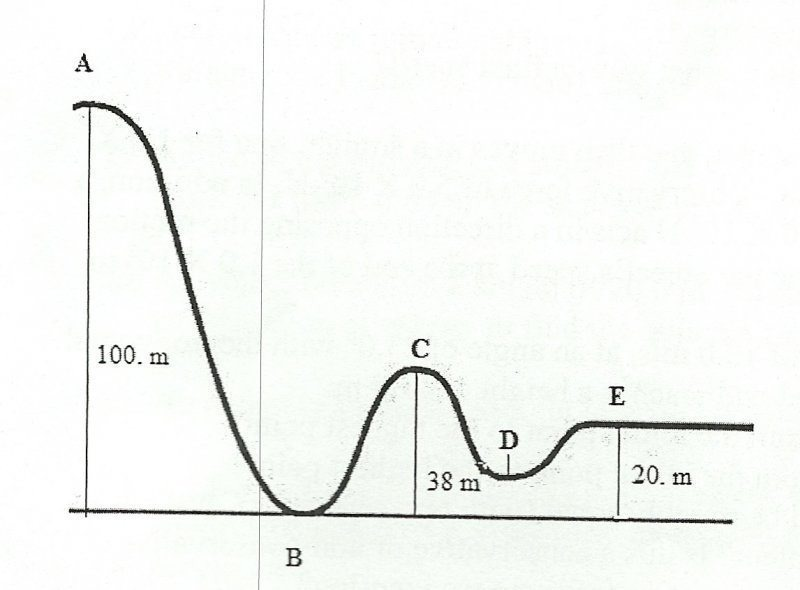
\includegraphics[scale=0.4]{roller-coaster}
\end{center}
\begin{enumerate}
\item Rank the points A through E from least to greatest potential Energy
\item Rank the points A through E from least to greatest kinetic Energy
\item At what point is the total energy entirely kinetic? (0 potential energy?)
\end{enumerate}

\vspace{2cm}
\textbf{Problem 2:} A pendulum is released from rest at point A.

\begin{center}
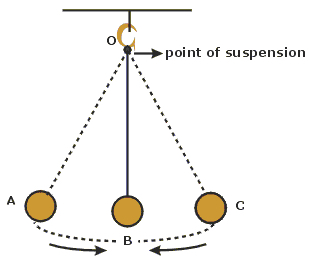
\includegraphics[scale=0.8]{pendulum}
\end{center}

\begin{enumerate}
\item Rank the points A through C from least to greatest potential energy
\item Rank the points A through C from least to greatest kinetic energy
\item At what point is the total energy entirely kinetic? (0 potential energy?)
\item Which points in the motion have the same potential energy?
\item Imagine a point halfway through the pendulum's motion from A to B. Describe where else in the pendulum's motion it would have the same kinetic energy as that first halfway point.
\end{enumerate}

\end{document}
